\begin{exercise}[19/1]

Betrachte den Shift-Operator $S$ am $\ell^2(\N)$, das ist

\begin{align*}
  S:
  \begin{cases}
    \ell^2(\N)              & \to     \ell^2(\N) \\
    (x_1, x_2, x_3, \ldots) & \mapsto (0, x_1, x_2, \ldots)
  \end{cases}
\end{align*}

\begin{enumerate}[label = (\alph*)]

  \item
  Zeige dass $S$ isometrisch ist, bestimme $\ran{S}$ und zeige dass $\ran{S}$ abgeschlossen ist, und zeige $\bigcap_{n=1}^\infty \ran{S^n} = \Bbraces{0}$.

  \item
  Bestimme die Hilbertraumadjungierte $S^\ast$ von $S$, und bestimme $\ker{(S^\ast)}$, $\ran{(S^\ast)}$, und $\bigcap_{n=1}^\infty \ran{[S^\ast]^n}$.

\end{enumerate}

\end{exercise}

\begin{solution}

\leavevmode \\

\begin{itemize}

  \item
  $S$ ist isometrisch:

  Klar.

  \item
  $\ran{S}$ abgeschlossen:

  \begin{align*}
    \ran{S}
    =
    \Bbraces
    {
      (x_n)_{n \in \N} \in \ell^2(\N):
      x_0 = 0
    }
  \end{align*}

  Sei $(\vv{x_n})_{n=0}^\infty = (S(\vv{y_n}))_{n=0}^\infty$ eine gegen $\vv{x}$ konvergente Folge aus $\ran{S}$.
  Weil $S$ isometrisch und linear ist, gilt $\| S(\vv{y_n}) - S(\vv{y_m})\| = \| S(\vv{y_n} - \vv{y_m}) \| = \| \vv{y_n} - \vv{y_m} \|$.
  Also ist auch $(\vv{y_n})_{n=0}^\infty$ eine Cauchyfolge in $\ell^2$ und damit konvergent gegen ein $\vv{y} \in \ell^2$.

  \begin{align*}
    \norm{S(\vv{y}) - \vv{x}}
    \leq
    \norm{S(\vv{y}) - S(\vv{y_n})} +
    \norm{S(\vv{y_n}) - \vv{x}}
    \xrightarrow{n \to \infty} 0
    \implies
    \vv{x} = S(\vv{y}) \in \ran{S}
  \end{align*}

  \item
  $\bigcap_{n=0}^\infty \ran{S^n} = \Bbraces{0}:$

  Für ein $(x_k)_{k \in \N} \in \ran{S^n}$ gilt $x_n = 0$.
  Liegt $(x_k)_{k \in \N}$ im Schnitt aller $\ran{S^n}$, ist also jede Komponente gleich Null.

  \item
  Wir bestimmen nun die Hilbertraumadjungierte $S^\ast$ von $S$.

  Es sei an folgende Definitionen erinnert.

  \begin{align*}
    S^\prime: \Bigg \{
    \begin{matrix}
      (\ell^2)^\prime &
      \to             &
      (\ell^2)^\prime, \\
      y^\prime        &
      \mapsto         &
      x \mapsto y^\prime(S(x)),
    \end{matrix}
    \quad
    S^\ast: \Bigg \{
    \begin{matrix}
      \ell^2           &
      \to              &
      \ell^2, \\
      (x_n)_{n \in \N} &
      \mapsto          &
      \Phi^{-1}(S^\prime(\Phi((x_n)_{n \in \N}))))
    \end{matrix}
  \end{align*}

  \begin{center}
  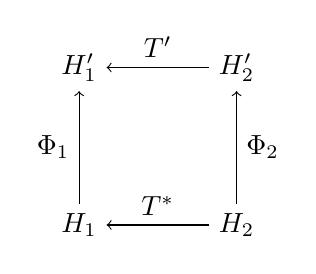
\begin{tikzpicture}[auto]
      \node (H1strich) at (0,0) {$H_1^{\prime}$};
      \node (H2strich) at (2,0) {$H_2^{\prime}$};
      \node (H1) at (0,-2) {$H_1$};
      \node (H2) at (2,-2) {$H_2$};
      \draw[->] (H2strich) to node [swap] {$T^{\prime}$} (H1strich);
      \draw[->] (H2) to node [swap]  {$T^*$} (H1);
      \draw[->] (H1) to node {$\Phi_1$} (H1strich);
      \draw[->] (H2) to node [swap] {$\Phi_2$} (H2strich);
  \end{tikzpicture} \\
  \end{center}

  $\ell^2$ ist isomorph zu seinem eigenen Dualraum $(\ell^2)^\prime$ vermöge folgender Abbildung.

  \begin{align*}
    \Phi: \Bigg \{
    \begin{matrix}
      \ell^2             &
      \rightarrow        &
      (\ell^2)^\prime \\
      (x_n)_{n \in \N}   &
      \mapsto            &
      ((y_n)_{n \in \N} \mapsto \sum_{n=0}^\infty y_n \overline{x_n})
    \end{matrix}
  \end{align*}

  Durch Anwendung dieser Definitionen erhalten wir

  \begin{align*}
    S^\ast((x_n)_{n \in \N})
    & =
    \Phi^{-1}(S^\prime(\Phi((x_n)_{n \in \N})))
    =
    \Phi^{-1} \pbraces
    {
      S^\prime \pbraces
      {
        (y_n)_{n \in \N}
        \mapsto
        \sum_{n=0}^\infty
        y_n \overline{x_n}
      }
    } \\
    & =
    \Phi^{-1} \pbraces
    {
      (y_n)_{n \in \N}
      \mapsto
      (0, y_0, y_1, y_2, \ldots)
      \mapsto
      0 \cdot x_0 +
      \sum_{n=0}^\infty
      y_n \overline{x_{n+1}}
    }
    =
    (x_{n+1})_{n \in \N}.
  \end{align*}

  Die Hilbertraumadjungierte $S^\ast$ macht also das \Quote{Gegenteil} von $S$.
  Sie verschiebt eine Folge um einen Eintrag nach links. \\

  \underline{Alternativ (und ohne Dualräume):} \\

  Die Hilbertraumadjungierte $S^\ast$ ist charakterisiert durch

  \begin{align*}
    (Sx, y)
    =
    (x, S^\ast y)
    \text{~für alle~}
    x \in \ell^2(\N)
    \implies
    0 + \sum_{n=2}^\infty x_{n-1} \overline{y_n}
    =
    \sum_{n=1}^\infty x_n \overline{y_{n+1}}
    \stackrel{!}{=}
    \sum_{n=1}^\infty x_n (S^\ast y)_n
  \end{align*}

  Die Hilbertraumadjungierte $S^\ast$ verschiebt eine Folge also um einen Eintrag nach links.

  \item
  \begin{align*}
    \ker{S^\ast}
    =
    \Bbraces
    {
      (c, 0, 0, 0, ...):
      c \in \C
    }
  \end{align*}

  %\item $\ran{S^\ast} = \ell^2$, denn es gilt $\sum_{n=0}^\infty |x_n|^2 < \infty \Longleftrightarrow \sum_{n=1}^\infty |x_n|^2 < \infty$.\textbf{Das folgt eh aus dem nächsten}

  \item
  $\ran{S^\ast}$:

  Sei $(x_k)_{k=0}^\infty \in \ell^2$.
  Betrachte folgende Folge $(y_k)_{k \in \N} \in \ell^2$.

  \begin{align*}
  y_k =
  \begin{cases}
    0,       & \text{falls~} k < n, \\
    x_{k-n}, & \text{falls~} k \geq n
  \end{cases}
  \end{align*}

  Diese erfüllt offenbar $(S^\ast)^n ((y_k)_{k=0}^\infty) = (x_k)_{k=0}^\infty$.
  Damit gilt $\Forall n \in \N:$

  \begin{align*}
    \ran{(S^\ast)^n}
    =
    \ell^2.
  \end{align*}

  \item
  \begin{align*}
    \bigcap_{n=0}^\infty
    \ran{(S^\ast)^n}
    =
    \ell^2
  \end{align*}

\end{itemize}

\end{solution}
